\chapter{Your 90-Day Automation Action Plan}


\section{Introduction}

Welcome to your 90-day automation journey! This chapter will guide you through a comprehensive action plan to transform your IT consulting practice through automation. We'll break down the next three months into manageable bi-weekly segments, each building upon the last to help you progressively enhance your automation skills and deliver tangible results for your clients.

Throughout this journey, we'll focus on leveraging the key tools we've explored in this book: n8n for workflow automation, NoCoDB for database management, and BudiBase for creating custom applications. We'll also incorporate other complementary tools as needed to create a well-rounded automation toolkit.

Remember, the goal isn't just to learn these tools in isolation, but to apply them to real-world problems and create meaningful automations for your clients. By the end of these 90 days, you'll have completed several automation projects, integrated multiple systems, and significantly enhanced your capabilities as an IT consultant.

Let's start by outlining our key objectives for this 90-day plan:

\begin{itemize}
    \item Complete at least 6 automation projects (one every two weeks)
    \item Integrate at least 3 different systems or tools
    \item Achieve measurable improvements in efficiency (time saved) and client satisfaction
    \item Overcome common technical challenges in implementation and data integration
    \item Build a portfolio of successful automations to showcase to potential clients
\end{itemize}

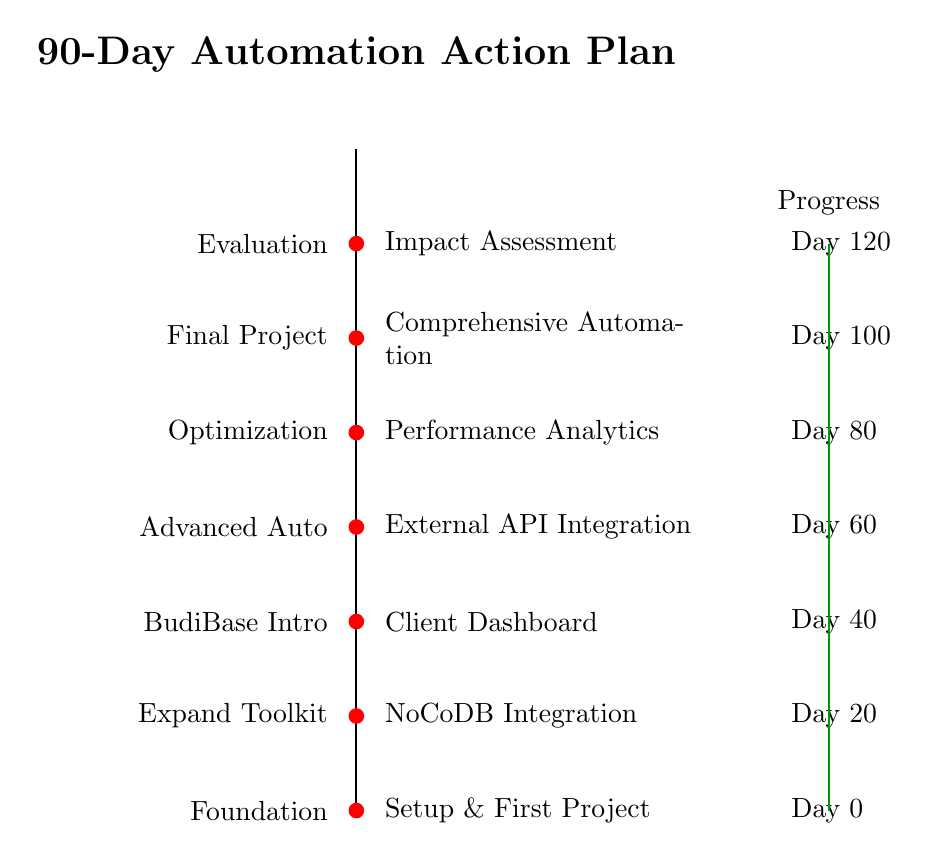
\begin{tikzpicture}[scale=1.2]
    % Title
    \node[font=\Large\bfseries] at (0,8) {90-Day Automation Action Plan};

    % Vertical timeline
    \draw[thick] (0,0) -- (0,7);

    % Milestones and phases
    \foreach \y/\day/\milestone/\phase in {
        0/0/Foundation/{Setup \& First Project},
        1/20/{Expand Toolkit}/{NoCoDB Integration},
        2/40/{BudiBase Intro}/{Client Dashboard},
        3/60/{Advanced Auto}/{External API Integration},
        4/80/Optimization/{Performance Analytics},
        5/100/{Final Project}/{Comprehensive Automation},
        6/120/Evaluation/{Impact Assessment}
    } {
        \node[circle, fill=red, inner sep=2pt] at (0,\y) {};
        \node[left, text width=3cm, align=right] at (-0.2,\y) {\milestone};
        \node[right, text width=4cm, align=left] at (0.2,\y) {\phase};
        \node[right] at (4.5,\y) {Day \day};
    }

    % Progress bar
    \draw[thick, green!60!black] (5,0) -- (5,6);
    \node[above] at (5,6.2) {Progress};
\end{tikzpicture}


\section{Weeks 1-2: Foundation and First Automation}

\subsection{Objectives}
\begin{itemize}
    \item Set up your automation environment
    \item Complete your first basic automation project
    \item Establish baseline metrics for time spent on manual tasks
\end{itemize}

\subsection{Action Steps}

\subsubsection{Step 1: Environment Setup}
Begin by setting up your automation toolkit:

\begin{itemize}
    \item Install and configure n8n locally or set up a cloud instance
    \item Set up a NoCoDB instance for data management
    \item Install BudiBase for creating custom applications
\end{itemize}

% TODO @screenshot: Show the setup screens for n8n, NoCoDB, and BudiBase side by side

\subsubsection{Step 2: Identify Your First Automation Project}
Choose a simple, high-impact task to automate. Consider starting with one of these:

\begin{itemize}
    \item Automate email responses for common client inquiries
    \item Create a simple task management system
    \item Set up automated reporting for a client project
\end{itemize}

\subsubsection{Step 3: Implement Your First Automation}
Use n8n to create a workflow for your chosen task. Here's a basic example of an automated email response system:

\begin{tikzpicture}[node distance=3cm, auto]
            % Define styles
    \tikzstyle{process} = [rectangle, minimum width=3.5cm, minimum height=1.2cm, text centered, draw=black, fill=blue!20]
    \tikzstyle{decision} = [diamond, minimum width=4cm, minimum height=2cm, text centered, draw=black, fill=green!20]
    \tikzstyle{arrow} = [thick,->,>=stealth]

    % Nodes
    \node (start) [process] {Email Received};
    \node (check) [decision, below of=start, yshift=-2cm] {Check Content};
    \node (auto) [process, below left of=check, xshift=-2cm, yshift=-2cm] {Send Auto-Response};
    \node (forward) [process, below right of=check, xshift=2cm, yshift=-2cm] {Forward to Team};
    \node (end) [process, below of=check, yshift=-5cm] {Mark as Handled};

    % Arrows
    \draw [arrow] (start) -- (check);
    \draw [arrow] (check) -- node[left, xshift=-0.5cm] {Common Query} (auto);
    \draw [arrow] (check) -- node[right, xshift=0.5cm] {Complex Issue} (forward);
    \draw [arrow] (auto) |- (end);
    \draw [arrow] (forward) |- (end);
\end{tikzpicture}

\subsubsection{Step 4: Measure and Record Baseline Metrics}
Before fully implementing your automation, measure how long the task takes manually. Record this in your progress tracker. This will be crucial for demonstrating the value of your automation efforts later.

\subsection{Check-In and Reflection}
At the end of week 2, reflect on your progress:

\begin{itemize}
    \item Did you successfully set up your environment?
    \item Have you completed your first automation project?
    \item What challenges did you face, and how did you overcome them?
\end{itemize}


\section{Weeks 3-4: Expanding Your Toolkit}

\subsection{Objectives}
\begin{itemize}
    \item Integrate NoCoDB into your automation workflows
    \item Complete a more complex automation project
    \item Start measuring time saved through automation
\end{itemize}

\subsection{Action Steps}

\subsubsection{Step 1: NoCoDB Integration}
Enhance your existing automation or create a new one that incorporates NoCoDB:

\begin{itemize}
    \item Set up a database in NoCoDB to store client information or project data
    \item Use n8n to create a workflow that reads from or writes to your NoCoDB database
\end{itemize}

% TODO @screenshot: n8n workflow showing integration with NoCoDB

\subsubsection{Step 2: Implement a More Complex Automation}
Build upon your skills to create a more sophisticated automation. Some ideas:

\begin{itemize}
    \item Automate client onboarding process
    \item Create a system for automated time tracking and invoicing
    \item Set up a workflow for collecting and analyzing client feedback
\end{itemize}

\subsubsection{Step 3: Measure Time Savings}
Start tracking the time saved by your automations:

\begin{itemize}
    \item Compare the time taken for manual processes vs. automated ones
    \item Record these metrics in your progress tracker
    \item Calculate the potential time savings if applied across all your clients
\end{itemize}

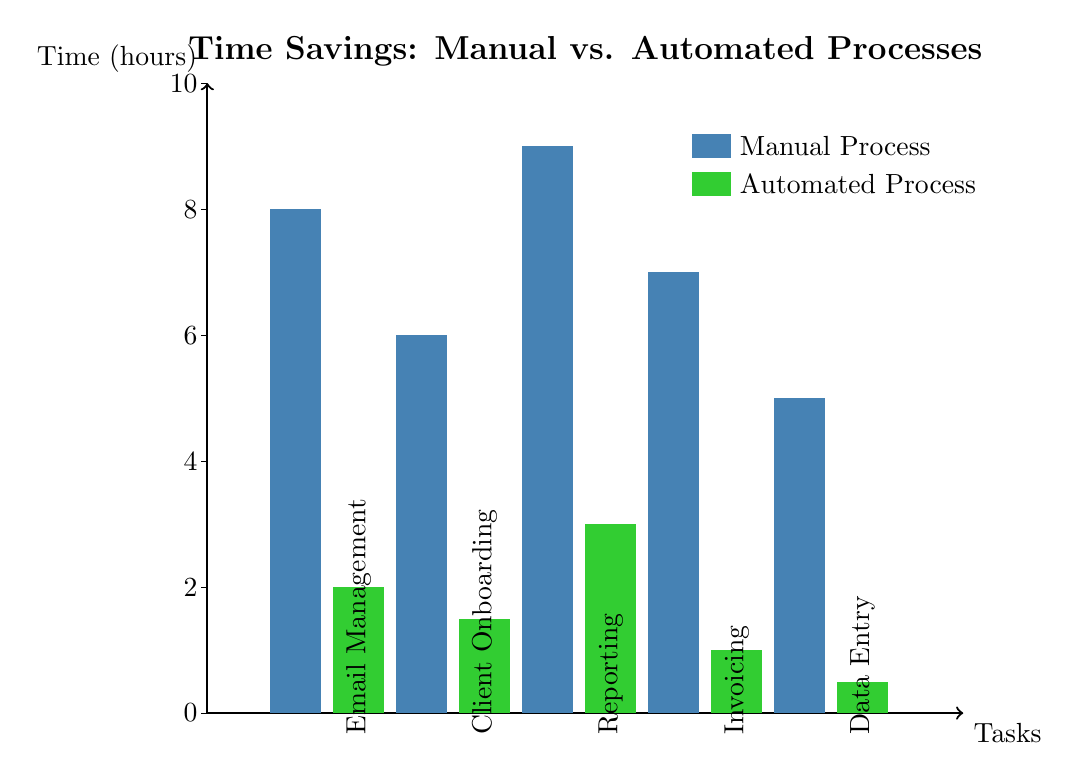
\begin{tikzpicture}[scale=0.8]
            % Define colors
    \definecolor{manualcolor}{RGB}{70,130,180}
    \definecolor{autocolor}{RGB}{50,205,50}

    % Y-axis
    \draw[thick,->] (0,0) -- (0,10) node[anchor=south east] {Time (hours)};
    \foreach \y in {0,2,4,6,8,10}
    \draw (0,\y) node[anchor=east] {\y} -- (-0.1,\y);

    % X-axis
    \draw[thick,->] (0,0) -- (12,0) node[anchor=north west] {Tasks};

    % Bars
    \foreach \x/\manual/\auto/\task in {
        1/8/2/Email Management,
        3/6/1.5/Client Onboarding,
        5/9/3/Reporting,
        7/7/1/Invoicing,
        9/5/0.5/Data Entry
    } {
        \fill[manualcolor] (\x,0) rectangle (\x+0.8,\manual);
        \fill[autocolor] (\x+1,0) rectangle (\x+1.8,\auto);
        \node[rotate=90, anchor=west] at (\x+1.4,-0.5) {\task};
    }

    % Legend
    \node[manualcolor, fill, rectangle, minimum width=0.5cm, minimum height=0.3cm] at (8,9) {};
    \node[right] at (8.3,9) {Manual Process};
    \node[autocolor, fill, rectangle, minimum width=0.5cm, minimum height=0.3cm] at (8,8.4) {};
    \node[right] at (8.3,8.4) {Automated Process};

    % Title
    \node[font=\large\bfseries] at (6,10.5) {Time Savings: Manual vs. Automated Processes};
\end{tikzpicture}


\section{Weeks 5-6: Introducing BudiBase and Enhancing Client Interaction}

\subsection{Objectives}
\begin{itemize}
    \item Create your first BudiBase application
    \item Integrate BudiBase with your existing automations
    \item Implement a client-facing dashboard or tool
\end{itemize}

\subsection{Action Steps}

\subsubsection{Step 1: BudiBase Basics}
Start by creating a simple application in BudiBase:

\begin{itemize}
    \item Design a basic client management or project tracking app
    \item Connect it to your NoCoDB database for data storage
    \item Familiarize yourself with BudiBase's UI components and logic
\end{itemize}

% TODO @screenshot: Simple BudiBase application interface

\subsubsection{Step 2: Integrate BudiBase with n8n}
Enhance your automation by connecting BudiBase and n8n:

\begin{itemize}
    \item Use n8n to trigger actions in your BudiBase app
    \item Create workflows that respond to events in your BudiBase application
\end{itemize}

\subsubsection{Step 3: Create a Client-Facing Tool}
Develop a tool or dashboard that provides value directly to your clients:

\begin{itemize}
    \item Design a project status dashboard
    \item Create a self-service portal for common client requests
    \item Implement a reporting tool that automatically generates and sends reports to clients
\end{itemize}

% TODO @screenshot: Client-facing dashboard created with BudiBase


\section{Weeks 7-8: Advanced Automation and Integration}

\subsection{Objectives}
\begin{itemize}
    \item Implement more advanced n8n features
    \item Integrate with external APIs or services
    \item Create a complex, multi-step automation workflow
\end{itemize}

\subsection{Action Steps}

\subsubsection{Step 1: Explore Advanced n8n Features}
Dive deeper into n8n's capabilities:

\begin{itemize}
    \item Experiment with error handling and retry mechanisms
    \item Use n8n's looping features for batch processing
    \item Implement conditional workflows for more complex logic
\end{itemize}

\subsubsection{Step 2: External API Integration}
Expand your automation capabilities by integrating with external services:

\begin{itemize}
    \item Connect to a CRM system like Salesforce or HubSpot
    \item Integrate with project management tools like Jira or Trello
    \item Implement automation with cloud storage services like Google Drive or Dropbox
\end{itemize}
\begin{tikzpicture}[node distance=2cm, auto]
            % Define styles
    \tikzstyle{process} = [rectangle, minimum width=2.5cm, minimum height=1cm, text centered, draw=black, fill=blue!20]
    \tikzstyle{decision} = [diamond, minimum width=3cm, minimum height=1cm, text centered, draw=black, fill=green!20]
    \tikzstyle{io} = [trapezium, trapezium left angle=70, trapezium right angle=110, minimum width=3cm, minimum height=1cm, text centered, draw=black, fill=red!20]
    \tikzstyle{cloud} = [ellipse, minimum width=3cm, minimum height=1cm, text centered, draw=black, fill=orange!20]
    \tikzstyle{arrow} = [thick,->,>=stealth]

    % Nodes
    \node (start) [cloud] {Start};
    \node (trigger) [io, below of=start] {Email Trigger};
    \node (parse) [process, below of=trigger] {Parse Email};
    \node (decision) [decision, below of=parse, yshift=-1cm] {Type?};
    \node (crm) [cloud, below left of=decision, xshift=-2cm, yshift=-1cm] {CRM (Salesforce)};
    \node (pm) [cloud, below of=decision, yshift=-1cm] {PM (Jira)};
    \node (storage) [cloud, below right of=decision, xshift=2cm, yshift=-1cm] {Storage (Dropbox)};
    \node (update) [process, below of=pm, yshift=-1cm] {Update Database};
    \node (report) [process, below of=update] {Generate Report};
    \node (send) [io, below of=report] {Send Notification};
    \node (end) [cloud, below of=send] {End};

    % Arrows
    \draw [arrow] (start) -- (trigger);
    \draw [arrow] (trigger) -- (parse);
    \draw [arrow] (parse) -- (decision);
    \draw [arrow] (decision) -- node[left] {Lead} (crm);
    \draw [arrow] (decision) -- node[right] {Task} (pm);
    \draw [arrow] (decision) -- node[right] {Document} (storage);
    \draw [arrow] (crm) |- (update);
    \draw [arrow] (pm) -- (update);
    \draw [arrow] (storage) |- (update);
    \draw [arrow] (update) -- (report);
    \draw [arrow] (report) -- (send);
    \draw [arrow] (send) -- (end);

    % External API labels
    \node [text width=3cm, text centered, above of=crm, yshift=-0.5cm] {Salesforce API};
    \node [text width=3cm, text centered, above of=pm, yshift=-0.5cm] {Jira API};
    \node [text width=3cm, text centered, above of=storage, yshift=-0.5cm] {Dropbox API};

    % Database
    \node (db) [cylinder, shape border rotate=90, draw, minimum height=2cm, minimum width=1cm, fill=yellow!20, right of=update, xshift=3cm] {NoCoDB};
    \draw [arrow, dashed] (update) -- (db);
    \draw [arrow, dashed] (db) -- (report);

    % Title
    \node[font=\large\bfseries] at (0,-11) {Complex n8n Workflow with Multiple Integrations};
\end{tikzpicture}


\section{Weeks 9-10: Optimization and Scaling}

\subsection{Objectives}
\begin{itemize}
    \item Optimize existing automations for better performance
    \item Implement analytics to track automation effectiveness
    \item Prepare automations for scaling across multiple clients
\end{itemize}

\subsection{Action Steps}

\subsubsection{Step 1: Performance Optimization}
Review and enhance your existing automations:

\begin{itemize}
    \item Identify and eliminate bottlenecks in your workflows
    \item Implement caching strategies where appropriate
    \item Optimize database queries in NoCoDB
\end{itemize}

\subsubsection{Step 2: Implement Analytics}
Set up systems to track the effectiveness of your automations:

\begin{itemize}
    \item Use n8n to log key events and metrics
    \item Create a dashboard in BudiBase to visualize automation performance
    \item Set up alerts for potential issues or anomalies
\end{itemize}

% TODO @screenshot: Analytics dashboard in BudiBase showing automation performance metrics


\section{Weeks 11-12: Final Project and Evaluation}

\subsection{Objectives}
\begin{itemize}
    \item Complete a comprehensive automation project
    \item Evaluate the overall impact of your automation journey
    \item Prepare to showcase your work to potential clients
\end{itemize}

\subsection{Action Steps}

\subsubsection{Step 1: Final Automation Project}
Put all your skills together in a final, comprehensive project:

\begin{itemize}
    \item Choose a complex business process to automate fully
    \item Incorporate n8n, NoCoDB, and BudiBase in your solution
    \item Implement advanced features like error handling, scalability, and analytics
\end{itemize}

\subsubsection{Step 2: Comprehensive Evaluation}
Assess the impact of your 90-day automation journey:

\begin{itemize}
    \item Calculate total time saved across all your automation projects
    \item Evaluate improvement in task accuracy and consistency
    \item Gather feedback from team members or clients who have interacted with your automations
\end{itemize}

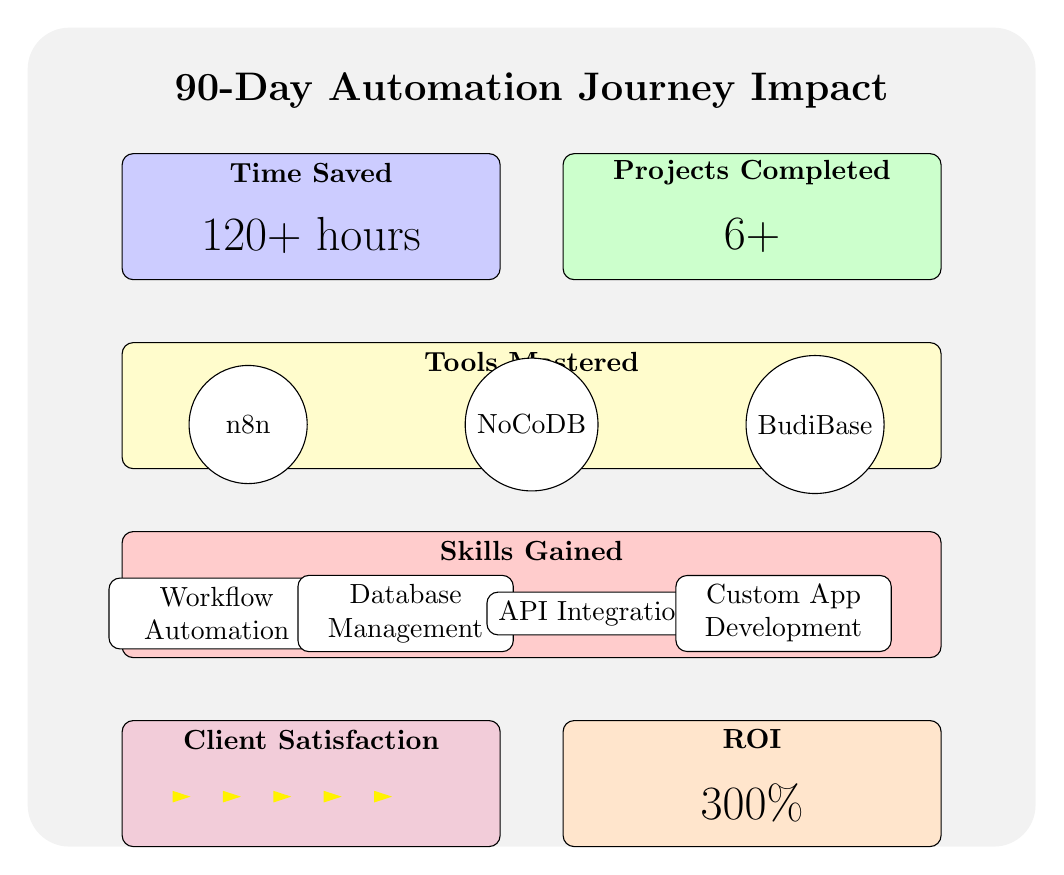
\begin{tikzpicture}[scale=0.8]
            % Background
    \fill[rounded corners=15pt, fill=gray!10] (-1,-1) rectangle (15,12);

    % Title
    \node[font=\Large\bfseries] at (7,11) {90-Day Automation Journey Impact};

    % Time Saved Section
    \begin{scope}[shift={(0.5,8)}]
    \draw[fill=blue!20, rounded corners] (0,0) rectangle (6,2);
    \node[font=\bfseries] at (3,1.7) {Time Saved};
    \node[font=\LARGE] at (3,0.7) {120+ hours};
    \end{scope}

    % Projects Completed Section
    \begin{scope}[shift={(7.5,8)}]
    \draw[fill=green!20, rounded corners] (0,0) rectangle (6,2);
    \node[font=\bfseries] at (3,1.7) {Projects Completed};
    \node[font=\LARGE] at (3,0.7) {6+};
    \end{scope}

    % Tools Mastered Section
    \begin{scope}[shift={(0.5,5)}]
    \draw[fill=yellow!20, rounded corners] (0,0) rectangle (13,2);
    \node[font=\bfseries] at (6.5,1.7) {Tools Mastered};
    \foreach \x/\tool in {2/n8n, 6.5/NoCoDB, 11/BudiBase} {
        \node[circle, fill=white, draw=black, minimum size=1.5cm] at (\x,0.7) {\tool};
    }
    \end{scope}

    % Skills Gained Section
    \begin{scope}[shift={(0.5,2)}]
    \draw[fill=red!20, rounded corners] (0,0) rectangle (13,2);
    \node[font=\bfseries] at (6.5,1.7) {Skills Gained};
    \foreach \x/\skill in {
        1.5/Workflow Automation,
        4.5/Database Management,
        7.5/API Integration,
        10.5/Custom App Development
    } {
        \node[draw, rounded corners, fill=white, text width=2.5cm, align=center] at (\x,0.7) {\skill};
    }
    \end{scope}

    % Client Satisfaction
    \begin{scope}[shift={(0.5,-1)}]
    \draw[fill=purple!20, rounded corners] (0,0) rectangle (6,2);
    \node[font=\bfseries] at (3,1.7) {Client Satisfaction};
    \foreach \x in {1,...,5} {
        \fill[yellow] (\x*0.8,0.7) -- ++ (18:0.3) -- ++ (162:0.3) -- cycle;
    }
    \end{scope}

    % ROI
    \begin{scope}[shift={(7.5,-1)}]
    \draw[fill=orange!20, rounded corners] (0,0) rectangle (6,2);
    \node[font=\bfseries] at (3,1.7) {ROI};
    \node[font=\LARGE] at (3,0.7) {300\%};
    \end{scope}
\end{tikzpicture}


\section{Conclusion}

Congratulations on completing this 90-day automation action plan! You've come a long way, from setting up your first basic automation to implementing complex, multi-tool solutions that can significantly impact your IT consulting practice.

Remember, this is not the end, but rather the beginning of your journey as an automation-focused IT consultant. The field of automation is constantly evolving, and there will always be new tools, techniques, and challenges to explore.

As you move forward, remember that the true value of automation lies not just in the time and effort saved, but in the enhanced value you can provide to your clients. Use your new skills to deliver more strategic, impactful solutions that drive real business outcomes.

\textbf{Action Item}: Take the workflow we built in this chapter and customize it for your own business. What other steps could you add to make your client onboarding even more efficient?

% TODO @qr: QR code linking to additional resources and community support for ongoing automation learning